\section{Implementaciones}\label{sec:impl}

En esta sección se presenta una familia de implementaciones de \setchain de mundo
real construídas sobre Tendermint. 
%
En particular, se exponen tres implementaciones diferentes, comenzando con una
implementación inocente pero trivialmente correcta, y finalizando con una algoritmo
complejo que implementa \setchain utilizando funciones hash.
%

Para evitar repeticiones, las definciones de funciones que permanezcan sin cambios
de una versión a la siguiente, no serán re-escritas. Solo se volverán a presentar
aquellas funciones para las cuales la definición se vea modificada.
%
A su vez, con la intención de mantener consistencia en la nomenclatura, el término \textit{transacción}
se utiliza siempre para referirse a las \textit{transacciones de Tendermint}, mientras
que \textit{elemento} queda reservado para elementos a agregarse a la \setchain.
%
Dependiendo de la implementación, una transacción de Tendermint puede contener uno
o más elementos a ser agregados.


% \subsection{General Considerations about Implementation}\label{subsec:general}
Las implementaciones correctas de \setchain implementan dos métodos~(ver sección
~\ref{sec:setchain}): \Add y \Get y, por lo tanto, cada implementación provee definiciones
para ambas.
%

Tendermint provee dos \textit{endpoints} RPC principales: \texttt{Tendermint.Broadcast}
inyecta una transacción con el objetivo de que se haga \textit{commit} sobre ella, y
\texttt{Tendermint.Query} consulta el estado de la aplicación.
%

Por lo tanto, desde el punto de vista del cliente de la \setchain, solo existen dos
métodos (\Add y \Get).
%
Sin embargo, hay dos métodos adicionales que se utilizan para comunicarse con la
red de Tendermint subyacente (los ya mencionados \texttt{Tendermint.Broadcast} y
\texttt{Tendermint.Query}).
%

Finalmente, \setchain asume que hay un predicado definido por el usuario que define
cuándo un elemento es válido para ser admitido en el conjunto.
%
En esta sección, dicho predicado se referencia con la función \isValidElement.

%
A continuación se presentan diferentes definiciones de métodos y funciones de
modo que la aplicación corriendo sobre Tendermint implemente \setchain.

%
Como se mencionó en la sección previa ~(ver sección ~\ref{sec:prelim}), para la
implementación es necesario definir las distintas instancias de Tendermint ABCI
y los métodos presentados como parte de la API de \setchain.

\section{Primera implementación: vainilla}\label{sec:vanilla}

% Vanilla API - alg0
\begin{figure}[t!]
  \begin{adjustbox}{minipage=[t]{\columnwidth}}
    \begin{algorithm}[H]
      \renewcommand{\thealgorithm}{API Vanilla}         
      \caption{}%
      \label{alg:api-vanilla}%
      \small
      \begin{algorithmic}[1]
            \Function{\<add>}{$transaction$}\label{alg:van_add}
                \State \textbf{return} \<broadcastTx>($transaction$)
                % \Comment {Hit broadcast\_tx\_async RPC endpoint}.
            \EndFunction
      
            \Function{\<get>}{\null}\label{alg:van_get}
                	\State \textbf{return} \<abciquery>()
            \EndFunction
            
        \end{algorithmic}
      \end{algorithm}
	\end{adjustbox}
  \end{figure}

%
En el Algoritmo~\ref{alg:api-vanilla} se muestra la solución más sencilla a la API
de \setchain utilizando Tendermint.
%

Los clientes agregan elementos invocando (indirectamente) a la función
\texttt{Tendermint.Broadcast}, mientras que pueden consultar el estado actual de
la \setchain invocando (también de forma indirecta) a \texttt{Tendermint.Query}.
%

Para dar una implementación completa de \setchain utilizando Tendermint, además se
debe definir la aplicación ABCI (ver sección~\ref{subsec:abci}). 
%

El Algoritmo~\ref{alg:abci-vanilla} muestra la definición de la ABCI para la versión
Vainilla.
%
Solo se definen \CheckTx, \DeliverTx, y \EndBlock; el resto tiene implementaciones
triviales.

%
El flujo usual de elementos agregados por \Add(e) en esta implementación es el siguiente.
%
Primero Tendermint chequea que el elemento $e$ a agregar es válido a través de
\CheckTx, y si es correcto, entonces insertará el elemento en la mempool.
%
Luego de un tiempo, es esperable que el elemento $e$ sea añadido a un bloque de Tendermint,
y cuando se haga \textit{commit} sobre el bloque en el consenso, Tendermint enviará
la secuencia correspondiente de pedidos: \BeginBlock para indicar el inicio de un nuevo bloque,
una lista de llamadas a \DeliverTx por cada transacción agregada, \EndBlock para indicar la
finalización del bloque, y \Commit para señalizar que el estado puede ser persistido.


% Vanilla ABCI - alg1
\begin{figure}[t!]
  \begin{adjustbox}{minipage=[t]{\columnwidth}}
    \begin{algorithm}[H]
      \renewcommand{\thealgorithm}{ABCI Vanilla}         
      \caption{}%
      \label{alg:abci-vanilla}%
      \small
      \begin{algorithmic}[1]
            \State \textbf{Init:} \texttt{epoch} $\leftarrow$ \textbf{-1}, \texttt{next\_epoch} $\leftarrow$ \textbf{0}, \texttt{history} $\leftarrow$ \{\}, \texttt{the\_set} $\leftarrow$ \{\}

            \Function{\<CheckTx>}{$transaction$}\label{alg:van_check_tx}
                \State \textbf{return} \Call{\<isValidTransaction>}{$transaction$}
            \EndFunction
      
            \Function{\<DeliverTx>}{$transaction$}\label{alg:van_deliver_tx}
                \State \<element> $\leftarrow$ \Call{\<getElementFromTransaction>}{$transaction$}
                \If {\Call{\<isValidTransaction>}{$transaction$} and not \texttt{element} in \texttt{history}}
                    \State \texttt{the\_set} \(<- \, \texttt{the\_set} \cup \{\<element>\}\) \label{lst:line:blah2} \label{line:abci-vanilla-set}
                		\State  \texttt{history[next\_epoch]} \(<- \, \texttt{history}[\texttt{next\_epoch}] \cup \{\<element>\}\) \label{line:abci-vanilla-history}
                	\EndIf
                	\State \textbf{return}
            \EndFunction
            
            \Function{\<EndBlock>}{\null}\label{alg:van_end_block}
            		\State \texttt{hash} $\leftarrow$ \<Hash>(\texttt{history[next\_epoch]}, \texttt{next\_epoch})
            		\Comment{Calcular el hash de la época.}
                \State \texttt{epochProof} $\leftarrow$  \texttt{Sign(\texttt{hash}, PRIVATE\_KEY})
                \State \Call{\<add>}{\texttt{epochProof}}
                \State \(\<epoch>  <- \, \texttt{next\_epoch}\)
                \State \texttt{next\_epoch} \( \, <- \texttt{next\_epoch} + 1\)
                \Comment{Cada bloque de Tendermint define una época.}
                \State \textbf{return}
            \EndFunction
            
             \Function{\<Query>}{\null}\label{alg:van_query}
                \State \textbf{return} (\texttt{the\_set}, \texttt{history} up to \texttt{epoch}, \texttt{epoch})            
             \EndFunction
            
            \Function{\<isValidTransaction>}{$transaction$}\label{alg:van_is_valid_tx}
                \State \<element> $\leftarrow$ \Call{\<getElementFromTransaction>}{$transaction$}
                \State \textbf{return} \<isValidElement>(\<element>)
            \EndFunction
            
            \Function{\<getElementFromTransaction>}{$transaction$}\label{alg:van_get_element}
                \State \textbf{return} $transaction$
            \EndFunction
        \end{algorithmic}
      \end{algorithm}
	\end{adjustbox}
  \end{figure}


\begin{comment}

The usual flow of elements added by \<add>\((e)\) in the Vanilla implementation
is: first Tendermint checks that the element \(e\) is valid with \<CheckTx>, and if the
element is valid, then \(e\) is added to the mempool.
% The call to \texttt{Add(e)} will generate a request to
% \texttt{CheckTx()} to run validations over the element $e$.
% %
% If the element passes the validations, it is inserted to the mempool.
%
After a while, $e$ is expected to be added to a Tendermint block, and when the
block gets committed in the consensus, Tendermint sends first a \<BeginBlock>
request followed by a list of \<DeliverTx>, an \<EndBlock> request, and finally a
\<Commit>.
% requests (one for each transaction in the consented order) sandwiched by
% \<BeginBlock> and \<EndBlock> requests, and followed by a Commit.
%

Tendermint invokes function \texttt{CheckTx} to decide
whether a new transaction should be added to the mempool or discarded.
%
In this version, checking that a transaction is valid consists on simply
checking the validity of the element, as transactions contain only one
element.
%
%Commented the following line as I'm not sure about talking about future implementations
%in this subsection:
%However, in the following implementation transaction are not the same as
%elements.
%
% It may seem silly to define the \texttt{getElementFromTransaction()} function in
% this case (given that it has no effect, it is the identity function).
%
% However, the decision to explicitly define such a function is to reinforce the
% conceptual difference between a Tendermint transaction, and the elements to be
% added to the \setchain.

%

%The Tendermint consensus doesnt invoke the deliverTx
Tendermint core sends \texttt{DeliverTx} requests
asynchronously (but in order) once per each transaction in the block.
%
Transactions have already been ordered in the global consensus by
the Tendermint protocol when \texttt{DeliverTx} is executed.
%
For this algorithm, the only thing to do when transactions are delivered is to add
the underlying element to the \setchain only if it is a valid one.
% Should we mention Byzantine proposers here?
We cannot avoid checking if a transaction is valid because it may have been
valid by the time it was inserted in the mempool but rendered invalid by the
time is consolidated.
%
Additionally, a Byzantine node may add transactions without checking their
validity.
% If the element is not valid, the corresponding transaction should have been
% rejected by the mempool, but may have been included in a block by a Byzantine
% proposer.
%
Tendermint invokes function \texttt{EndBlock} once per block, after delivering
all transactions inside the block.
%
In this algorithn, the end of a block triggers an epoch increment, and thus,
each Tendermint block defines a different \setchain epoch.
%
Finally, when clients request a \texttt{Get}, they call the \<abciquery>
function.

\subsubsection{Elements Membership Proof}\label{subsubsec:membership}
%
Client processes do not know if they are contacting a Byzantine or correct
process.
%
To ensure that an element is going to be added to the \setchain, the client
needs to interact with enough servers to guarantee that at least one server is
correct~\cite{Capretto.2022.Setchain}.
%
% An extension to Setchain presented an optimistic client with the following
% approach.
%
Correct servers sign cryptographically a hash of the set of elements in an
epoch, and insert this hash in the \setchain as an element.
%
We call those hashes epoch proof elements. 
%
Epoch proofs may be implemented using Ed25519~\cite{ed25519} as signature system.
%
Epoch proofs may contain the epoch number being proved, the validator's public key
signing, and the signature of the elements in the given epoch (ordered in a well-known
specific way). 
%
Clients only perform a single $\<add>(e)$ request to one server, hoping it is a
correct server.
%
After waiting for some time, clients can invoke a \<get> from a single server
and checks whether $e$ is in some epoch and there exists enough epoch proofs\footnote{We
  assume that an upper bound, $f$, in the number of Byzantine servers is
  known and therefore $f+1$ signatures are required.} to guarantee that at
least one correct server has signed it.
% (at least) $f$ + 1 servers.
Clients are able to verify if epoch proofs are valid by generating the hash of elements
in the given epoch, and verifying if the signature in the epoch proof element is valid
for the hash and the public key.
%
Validators' public keys need to be publicly known to users.
%
If $e$ is in an epoch with enough epoch proofs, clients can conclude
that the epoch is correct and $e$ has been successfully inserted and
stamped.
%
Note that this requires only one message per \<add> and one message per \<get>.
%
We implemented this epoch proof mechanism in the definition of \<EndBlock>.

%
Another option to implement epoch proof elements is using ethereum crypto library.
%
This library provides a \texttt{Sign} function that calculates an ECDSA signature.
%
The produced signature is in the $[R || S || V]$ format, where $V$ is 0 or 1.
%
The $V$ value is usually called recovery bit, and it allows to use the \texttt{Ecrecover}
function, which takes in a hash and a signature, and returns the uncompressed public key
that created the given signature.
%
This way, epoch proof elements may contain the epoch number and the signature in the format
mentioned above, and clients may use the \texttt{Ecrecover} function to verify that the given
signature was indeed generated by a known validator.
%

%
Notice that epochs now contain two kind of elements: client regular elements, and epoch
proof elements; meaning that every epoch proof element belongs to an epoch. However,
epoch proof elements do not need to be included as elements in the signed hash that is
part of the epoch proof for the given epoch.
%
Consequently, we need to differentiate between regular elements, and epoch proof elements.
%
Regular elements are checked for validity using the already mentioned \texttt{isValidElement}
function.
%
However, an epoch proof element needs to be validated in other way: verifying the signature.
%

While the implementation described in this section implements \setchain, it is
not exploiting its main idea: to lift the total order between elements.
%
% and take advantage of the
% performance improvements that implies.
%
Even though several elements may belong to the same epoch, meaning that no total
order between them could be established, Tendermint consensus protocol is
running underneath deciding a total order for the elements.
% that then is broken
% when adding the elements from the same block to a specific epoch.


\subsection{Second Implementation: Compresschain}\label{subsec:compresschain}

To get closer to the specification of Setchain, we propose to pack elements
together into a batch, reassembling a set, and subsequently compressing it
prior to transmission.
%
We propose a new implementation, called \emph{Compresschain}, that attempts to
explore the relaxed order proposed by \setchain, even though we still run
Tendermint consensus underneath.
%
Instead of immediately broadcasting each element added by clients as a
Tendermint transaction, a new middleware piece of software called
\textit{collector} is responsible for collecting elements until reaching a batch
long enough and broadcast that batch as a transaction.
%
% This means that a new
% \setchain API version is defined, which uses the new collector component.
%
% We define a collector in Algorithm.

Following the current practice of Ethereum, we use Ethereum's Recursive Length
Prefix~\cite{ethereum} encoding and Brotli
compression~\cite{brotli.compressor}~\footnote{ Although other compressions
algorithms can be used if required.}.
%
% To achieve a better throughput in
% terms of size per element broadcasted,  is used.
%
Instead of adding elements sent by users into the network, we first collect them
and encode them using RLP, and once the batch is ready, we compress the batch
with the Brotli compression algorithm.
%
We do not provide any specific criteria to determine when batches are ready.
%
However, we have it depends on a maximum size as well as a reasonable amount of
time since the first element came in.
%
In Algorithm~\ref{alg:collector-brotli}, we show an implementation of a
collector algorithm, and in Algorithm~\ref{alg:api-brotli}, we present the new
\setchain API.
%
In this implementation, a client requesting an \<add> invokes the
collector \texttt{AddElement} method.
%, instead of \<broadcastTx>.
%
% Some simplifications were made, as for instance a race condition could occur if
% several routines add an element to the same collector instance at the same time.
% %
% However, that can be easily solved using locks.

% Compresschain API - 
\begin{figure}[t!]
  \begin{adjustbox}{minipage=[t]{\columnwidth}}
    \begin{algorithm}[H]
      \renewcommand{\thealgorithm}{API Compresschain}         
      \caption{}%
      \label{alg:api-brotli}%
      \small
      \begin{algorithmic}[1]
      
            \Function{\<add>}{$element$}\label{alg:brotli_add}
                \State \textbf{return} \texttt{CompressCollector.AddElement($element$)}
                \Comment {Usar el componente intermedio collector.}
            \EndFunction
      
            \Function{\<get>}{\null}\label{alg:brotli_get}
                	\State \textbf{return} \<abciquery>()
            \EndFunction
            
        \end{algorithmic}
      \end{algorithm}
	\end{adjustbox}
  \end{figure}


% Brotli Collector - alg2
\begin{figure}[t!]
  \begin{adjustbox}{minipage=[t]{\columnwidth}}
    \begin{algorithm}[H]
      \renewcommand{\thealgorithm}{Compress Collector}         
      \caption{}%
      \label{alg:collector-brotli}%
      \small
      \begin{algorithmic}[1]
            \State \textbf{Init:} \texttt{batch} $\leftarrow$ \{\}
      
            \Function{\<AddElement>}{$element$}\label{alg:brotli_add_tx}
            		\If {\<isValidElement>($element$)}
            			\State \texttt{encoded\_element} $\leftarrow$ \texttt{RLP.Encode}($element$)
					        \State \texttt{batch} $\leftarrow$ \texttt{batch} $\cup$ \{\texttt{encoded\_element}\}
                \EndIf
                \State \textbf{return}
            \EndFunction
            
            \smallskip

            \When {\<isReady>(\<batch>)}
              \State \texttt{compressed\_batch} $\leftarrow$  \texttt{Brotli.Compress}(\texttt{batch})
              \State \texttt{Tendermint.Broadcast}(\texttt{compressed\_batch}) \label{line:compresschain-broadcast}
              %\State \Call{\<reset>}{\null}
              \State \texttt{batch} $\leftarrow$ \{\}
            \EndWhen
            
            % \Function{\<reset>}{\null}\label{alg:brotli_reset}
            % 		\State \texttt{batch} $\leftarrow$ \{\}
            %     \State \textbf{return}
            % \EndFunction
        \end{algorithmic}
      \end{algorithm}
	\end{adjustbox}
  \end{figure}



%

% After the meeting we decided to call isValidElement() locally in the collector, so the following is not true:
% It is worth mentioning that, as the algorithm shows, the collector adds every element that receives to the batch without running any validation on it. While this clearly allows the batch to contain garbage, making a \textit{CheckTx()} request to the ABCI app for each new element would mean a decrease in performance, as the number of requests would keep constant in the number of elements sent by clients, instead of being constant in the number of batches, as it is desired.

%
To complete our definition, we provide the expected ABCI of Compresschain~(see
Algorithm~\ref{alg:abci-brotli}).
%
% There are some main differences as regards the previous \setchain implementation.

%
% Brotli ABCI - alg1
\begin{figure}[t!]
  \begin{adjustbox}{minipage=[t]{\columnwidth}}
    \begin{algorithm}[H]
      \renewcommand{\thealgorithm}{Compresschain ABCI}         
      \caption{\small }%
      \label{alg:abci-brotli}%
      \small
      \begin{algorithmic}[1]
            \State \textbf{Init:} \texttt{epoch} $\leftarrow$ \textbf{0}, \texttt{history} $\leftarrow$ \{\}

            \Function{\<CheckTx>}{$batch$}\label{alg:brotli_check_tx}
                \State \textbf{return} \Call{\<isValidBatch>}{$batch$}
            \EndFunction
      
            \Function{\<DeliverTx>}{$batch$}\label{alg:brotli_deliver_tx}
				\State \texttt{elements} $\leftarrow$ \Call{\<getElementsFromBatch>}{$batch$}
				\State \Call{\<newEpoch>}{\texttt{elements}}
            		
            		\State \textbf{return}
            \EndFunction
            
            \Function{\<isValidBatch>}{$batch$}\label{alg:brotli_is_valid}
            		\State elements $\leftarrow$ \Call{\<getElementsFromBatch>}{$batch$}
            		
            		\Comment{If at least one element in the batch is valid, then the batch is considered valid.}
            		\For{\texttt{e in} $elements$}
                    \If {\<isValidElement>(\texttt{e}) and not \texttt{e} in \texttt{history}}
                    		\State \textbf{return} \texttt{True}
                    \EndIf
                \EndFor
                \State \textbf{return} \texttt{False}
            \EndFunction
            
            \Function{\<getElementsFromBatch>}{$batch$}\label{alg:brotli_get_element}
                \State \texttt{decompressedBatch} $\leftarrow$ \texttt{Brotli.Decompress}($batch$)
                \State \texttt{elements} $\leftarrow$ \texttt{RLP.Decode}(\texttt{decompressedBatch})
                \State \textbf{return} \texttt{elements}
            \EndFunction
            
            \Function{\<newEpoch>}{$elements$}\label{alg:brotli_new_epoch}
            		\For{\texttt{e in} $elements$}
             		\If {\<isValidElement>(\texttt{e}) and not \texttt{e} in \texttt{history}}
                				\State \texttt{history[epoch]}.AddElement(e)
                				\Comment{Only add new valid elements.}
                    	 \EndIf
                	\EndFor
                	
                	\State \texttt{hash} $\leftarrow$ \<Hash>(\texttt{history[epoch]}, \texttt{epoch})
            		\Comment{Hash epoch (elements and number).}
                \State \texttt{epochProof} $\leftarrow$  \<Sign>(\texttt{hash}, privateKey)
                \State \Call{\<add>}{\texttt{epochProof}}
                	
                	\State \texttt{epoch} $\leftarrow$ \texttt{epoch} + 1
                \State \textbf{return}
            \EndFunction
        \end{algorithmic}
      \end{algorithm}
	\end{adjustbox}
  \end{figure}



The main difference with the Vainilla implementation is that transactions
contain potentially more than one element, because transactions are 
compressed batches of elements.
%
Moreover, to retrieve the elements inside transactions, we need to decompress
the batch first, and once the original batch is recovered, it has to be
RLP-decoded to get the original elements sent by the clients.
%
% Those original transactions corresponds to the elements to be added to
% the \setchain. \textit{getElementsFromTransaction()} function shows that
% behavior.

Using Compresschain, Tendermint transactions may contain both valid
and invalid elements.
%
We need to define a new criteria to define when a transaction is
considered valid.
%
The function \<isValidBatch>~(in Algorithm~\ref{alg:abci-brotli})
implements this new criteria, allowing transactions to be considered valid if at
least one element on it is valid.
%
The choice of this criteria is related to the fact that someone sending invalid
elements~\footnote{Elements may be valid at the moment clients send them, but
invalid when blocks are commited.} to a node should not prevent valid
elements sent to the same node from being added to the \setchain.
%
However, as it is illustrated in function \<DeliverTx>, only valid
elements are added to the \setchain, while invalid ones are simply discarded.

Finally, in Compresschain, blocks do not delimit epochs, and thus, we do not
give a definition to function \<EndBlock>.
%
In this case, we define epochs as transactions: each batch of elements defines an
epoch.
% %
% definition was given in this case, as the block does not
% delimit the epoch anymore, but the epoch is defined by all the elements
% belonging to the same Tendermint transaction.
% \textit{DeliverTx()} function
% shows the epoch number increase.

% To dicuss: if epochs are defined by batches, then epochs are generated by the same node.
% This is a new setchain property and may be undesirable. 
\subsection{Third Implementation: HashChain}\label{subsec:hashchain}
%
Hashchain aligns with the underlying concept introduced in Compresschain;
however, it uses hash functions rather than Brotli compression.
%Hashchain follows a similar idea introduced in Compresschain but employing hash
%functions instead of Brotli compression.
%
While the compression power of hash functions may be enormous, as those
functions map data of arbitrary size to fixed-size values, hashes are
irreversible, meaning that a non-trivial method to recover the original batch of elements
has to be provided.
%
The implementation of Hashchain involves two aspects: a Tendermint blockchain of
hashes and a distributed inverse function retrieving batches from hashes.
%
% We shouldn't mention "consolidated hashes" before explaining it:
%Therefore, we now have to maintain an inverse function for the consolidated
%hashes.

Often in this section we will take the liberty of referring to \textit{elements
in a hash H} for those elements belonging to a batch $B$, such that
$Hash(B) = H$.

Instead of using the compression collector as in Compresschain (see
Algorithm~\ref{alg:collector-brotli}), we now use a \emph{hash
collector}, where elements are batched and then hashed. 
%
Hashed batches are then added to the Tendermint network as transactions and
shared across the whole network, in a manner analogous to the approach employed
for compressed batches in Compresschain.

\subsubsection{Distributed Algorithm for Hash Reversal}

While the hash collector adopts a concept similar to the compression collector,
the ABCI side of Hashchain is considerably more complex.
%
In this scenario, \<CheckTx> as well as \<DeliverTx> receive hashes as a transaction.
%
The computer running the \setchain is not immediately able to translate
hashes into their original batch of elements, owing to the irreversible
nature of hashes.
%
The absence of the original batch of elements renders both \<CheckTx> incapable
of verifying the elements in the transaction and \<DeliverTx> unable to
add elements to the \setchain.
%

At this juncture, our distributed algorithm for hash reversal comes into play.
%
We need to communicate with a Tendermint node that knows the hash
(initially, only its creator).
%
To distribute the information about who knows the data of a hash, transactions
contain not only the hash of the batch but also a signature.
%
Signatures accompanying hashes indicate that a specific Tendermint
validator (the one signing the hash) claims to know the hash, hence,
if it is a correct node, it has the original batch of elements.
%
Then, transactions are represented by a tuple $(h, s)$, where $h$ denotes
the hash value and $s$ represents the signature obtained by signing $h$ with
the private key of the node that knows the hash.
%
Thanks to the signature, we can communicate with the node claiming to know the
data, and get the original batch, if the node behaves properly.
%
We can run the process of requesting hashes asynchronously to avoid potential
delays.

%

After leaving the hash collector, hashes are expected to be checked against
\<CheckTx> to be either added to the mempool or discarded.
%
To determine the validity of a hash, we need to check the elements in it.
%
Similar to Compresschain, hashes are considered valid if at least one element
in the hash is valid.
%
At the point \<CheckTx> runs, we cannot ensure that the original batch of
elements is known for the given instance.
%
Hashchain is optimistic in the sense that in the event of impossibility
to run the transaction check due to the absence of the original batch,
\<CheckTx> considers hashes as valid transactions with the hope that
their batches will be sent later on.

%
The optimistic nature of Hashchain entails notable consequences.
%
As the default behaviour for \<CheckTx> is to return \texttt{True},
we can have transactions in the blockchain without having the elements
but just the hash of the elements.
%
Moreover, a transaction may be committed without anyone having
previously checked it, but passing the check because of the optimistic
behavior.
%
For example, this is likely the case of the first time a new hash shows
up in the blockchain.

%

%Therefore, we need a way to extract the elements inside the transactions and
%provide the user a uniform view, that of a Setchain.
Therefore, we need to define the criteria by which a hash residing within the
blockchain is safe to be part of the \setchain.
% the HashChain living in
% Tendermint, and the \setchain we want to build.
%
To achieve that, we define a natural number \texttt{SIGNATURES\_PER\_HASH}
defining the number of signatures a hash has to possess to be considered a batch
of elements to be added to the \setchain.
%
We are only interested in hashes signed by at least
\texttt{SIGNATURES\_PER\_HASH} nodes, and we call them
%
% A hash for which the ABCI has seen \texttt{SIGNATURES\_PER\_HASH} or more
% signatures, it is said to be a
\textit{consolidated hashes}.
%
\texttt{SIGNATURES\_PER\_HASH} is defined in such a way that a consolidated hash
is guaranteed to be known by at least one correct node.
%
The elements of consolidated hashes are the candidates to belong to the
Setchain.

%Following the same criteria as in Compresschain, we consider a transaction to
%be valid if we can get the data and validate at least one of its elements.
%
% With this in mind, whenever the ABCI gets the revert of a hash, it runs the
% validation against it, and
%Moreover, if at least one element in the batch is valid, the node verifying the
Whenever a node asks for the revert of hash, if at least one element in the batch
is valid, the node signs the hash, and broadcast the hash along with its own signature.
%
By broadcasting the hash and its signature, the node announces to the network
that they know the data behind that hash.
%
This way, valid batches will eventually consolidate, meaning their elements will
be added to the \setchain.

For all this to work, we need to keep track of how many signatures a hash has,
as well as a map from hashes to batches.
%
Each time \<DeliverTx> gets a transaction, we check the
signature for validity.
%
If the signature is valid and new for the given hash, we increase the
\textit{signatures per hash} counter.
%
In addition, each time we revert a hash, we check the correctness of the
original batch (i.e $hash = Hash(originalBatch)$).
In case of success, the map from hashes to
batches is updated with the new discovery.

%The first time a hash is passed around, other nodes would see the new hash and
%try to get the data from other servers.
%
%The first one claiming to have the data is the creator of the transaction.


%When a \<get> arrives, we need to get the elements out of the consolidated
%hashes.
% it is necessary to ask for the batch
% corresponding to the hash in the transaction.
%



% Something we discussed with Marga: when the collector creates a hash h and signs it, and broadcast (h, s) every call to CheckTx(h, s) will be true, as no one is expected to have the reverse of h the first time they see it. Because of that, (h, s) in the hashchain doesn't mean that there is at least one good valid element in the h. h could be full of garbage
% A client could contact every collector node with the same elements, and every collector would broadcast (h, sn), with n being the n-collector. This could cause that hash h consolidates, without anyone really having checking elements in h. Is that bad? not too bad, only an empty epoch would occur. Possible fixes: collector hashes elements + pubkey, chain of signatures

\subsubsection{Consolidation Epoch}\label{subsubsec:consolidation}

In this implementation, epochs are defined by all the elements in a hash, similar to
Compresschain implementation.
%
In other words, elements from the same consolidated hash belong to the same
epoch.
%
%Now we have to be more careful when adding elements to the setchain, elements
%may appear several times depending on how nodes form batches and
%hashes. \marga{esto no puede pasar tambien en compresschain? un
%  elemento no puede aparecer en varios batches?}
%
% However, what epoch number is that? We need to be more specific
% to define this.

%

In this paper, we present two alternatives to assign an epoch to a consolidated
hash.
%
The first one is called \textit{Current Epoch Consolidation} (CEC), meaning that
once a hash consolidates, all their underlying elements are added to the current
epoch (i.e the epoch in which the \texttt{SIGNATURES\_PER\_HASH}-th signature
has been seen).
%
The second one, \textit{First Seen Epoch Consolidation} (FSEC) assigns the epoch
according to when the hash has been seen for the very first time, once
consolidated.
%
Transactions (hashes in this case) in Tendermint blocks are totally
ordered, so both strategies can determine which hash occurs or
consolidates first, and all correct nodes will agree on it.

%

In Figure~\ref{fig:consolidation_epoch}, we show an example of these two different
strategies to assign an epoch to a consolidated hash when
\texttt{SIGNATURES\_PER\_HASH} is 3.
%
Hash $j$ is the first hash in block $m$, and hash $k$ is the hash that first
consolidates (getting its third signature).
%
On one hand, current Epoch Consolidation strategy assigns the epoch as soon as the hash
consolidates, stamping elements from hash $k$ with epoch $a$ first, and then
elements from hash $j$ with epoch $a+1$.
%
On the other hand, First Seen Epoch Consolidation implementation does not assign the
epoch to hash $k$ just when it consolidates, because hash $j$ has been seen for first
time before hash $k$.
%
As hash $j$ consolidates right after hash $k$, elements from hash $j$ are
stamped with epoch $a$, and then elements from hash $k$ are stamped with epoch
$a+1$.

\begin{figure}
  \centering
  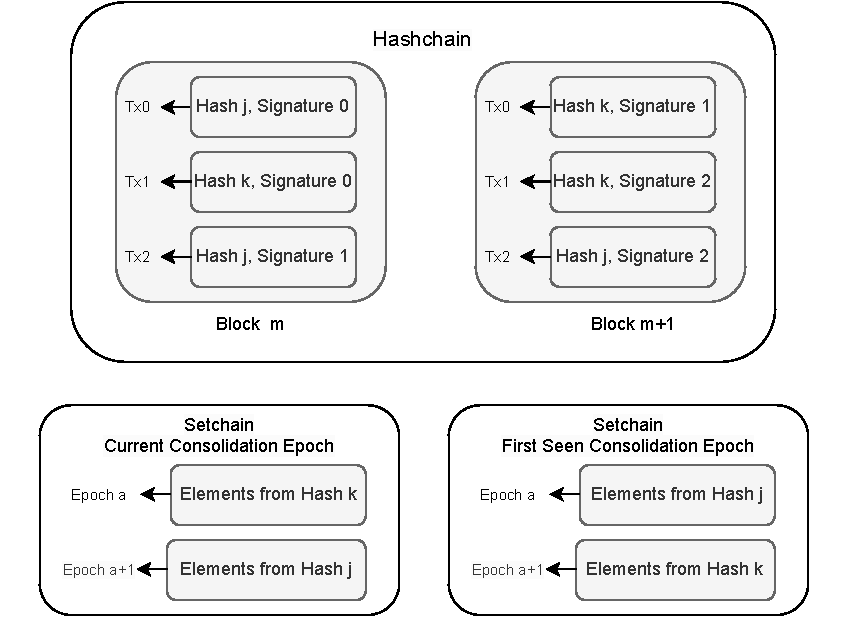
\includegraphics[scale=0.5]{figures/consolidation_epoch.pdf}
  \caption{Consolidation epoch strategies}
  \label{fig:consolidation_epoch}
\end{figure}

First Seen Epoch Consolidation variant grants hashes a grace period in which
they can be either consolidated or rejected.
%
% The grace period is necessary, let
% us briefly examine why.
Assuming no grace period at all, if a hash $j$ occurs for
first time before hash $k$, once consolidated, elements from hash $j$ would be
stamped with epoch $E$, while elements from hash $k$ would be stamped with epoch
$F$ \textgreater \ $E$.
%
Hence, let $j$ be a hash first seen at a given moment such
that, once consolidated, it would be assigned the epoch $E$.
%
If hash $j$ never achieves the \texttt{SIGNATURES\_PER\_HASH} signatures to
consolidate, a newer hash $k$ (a hash first seen after $j$) would not be able to
consolidate, as its underlying elements could not be stamped with an epoch $F$
\textgreater \ $E$, if epoch $E$ was not defined yet.
%
In Figure~\ref{fig:grace_period}, we show an example of this.
%
We conclude that a grace period is necessary to guarantee the successful evolution of
the hashchain, as hashes $k$ and $l$ (and even $o$ and $q$) are not able to
consolidate until $j$ consolidates or gets rejected.


It is worth noting that the crucial aspect to consolidation in FSEC lies in the
occurrence of all \texttt{SIGNATURES\_PER\_HASH} signatures within a window
equivalent to the duration of the grace period.
%
Hashes that are initially rejected can consolidate in the future as long as
they reach the \texttt{SIGNATURES\_PER\_HASH} signatures within the grace period.
%
Hashes achieving the \texttt{SIGNATURES\_PER\_HASH}-th signature after
the grace period will not undergo consolidation in the current round;
however, they can do it in the future.

\begin{figure}
  \centering
  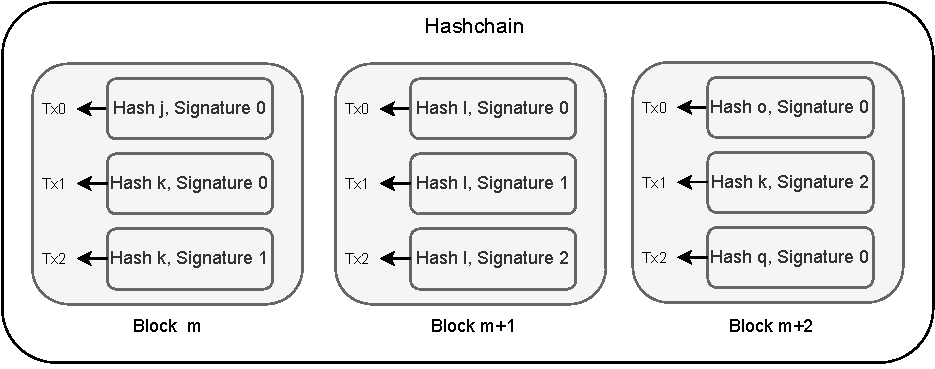
\includegraphics[scale=0.5]{figures/grace_period.pdf}
  \caption{Scenario requiring grace period under FSEC.}
  \label{fig:grace_period}
\end{figure}

%\subsubsection{Elements Membership Proof}
% Do not use this because we want a proof that specific elements belong to a specific epoch.
%Client processes do not know if they are contacting a Byzantine or correct process. The general idea of a client protocol that wants to ensure that an element is going to be added to the \setchain is to interact with enough servers to guarantee that some are correct. To guarantee contacting at least one correct server, the client needs to send f + 1 messages. However, each element added to the \setchain comes from a consolidated hash. That means that we already have \textbf{SIGNATURES\_PER\_HASH} validator's signatures for that hash. Those signatures may act as a proof for the batch of elements that really belongs to the \setchain. If that proof is added to the epoch as an extra element, a client sending an element, waiting for a while, and then requesting a Get to only one server (hoping it is correct server) may be sure that its element belongs to the \setchain because the epoch comes along a proof of their elements. 

% Setchain API - 
\begin{figure}[t!]
  \begin{adjustbox}{minipage=[t]{\columnwidth}}
    \begin{algorithm}[H]
      \renewcommand{\thealgorithm}{API Hashchain}         
      \caption{}%
      \label{alg:api-hashchain}%
      \small
      \begin{algorithmic}[1]
      
            \Function{\<add>}{$element$}\label{alg:hash_add}
                \State \textbf{return} \texttt{HashCollector.AddElement($element$)}
                \Comment {Use the middleware collector component}.
            \EndFunction
      
            \Function{\<get>}{\null}\label{alg:hash_get}
                	\State \textbf{return} \<abciquery>()
            \EndFunction
            
        \end{algorithmic}
      \end{algorithm}
	\end{adjustbox}
  \end{figure}


\subsubsection{Implementation details}\label{subsubsec:details}

We do not define a new collector for Hashcahin since it is similar to the one
define for Compresschain where the only difference is the use of hash functions.
%
% No collector piece for Hashchain appears as it is similar to the already
% presented collector for Brotli, employing hash functions instead of Brotli
% compression.
We define the Setchain API in Algorithm ~\ref{alg:api-hashchain}.
% shows how a new collector is
% used now in order to add elements to the \setchain.

Finally, as regards the ABCI, we show a possible implementation for Hashchain
with Current Epoch Consolidation strategy in Algorithm~\ref{alg:abci-hash1} and ~\ref{alg:abci-hash2}. It is
noteworthy that within the algorithm, the function \<Query> initiates the construction
of \<history>, in addition to broadcasting epoch proofs. Although this approach is employed
for clarity, a node that receives infrequent query requests may experiment delays in
generating the epoch proofs. As a result, the process of constructing \<history> and
epoch proofs can be scheduled periodically, independent of query requests.

% Hash ABCI - alg4
\begin{figure}[t!]
  \begin{adjustbox}{minipage=[t]{\columnwidth}}
    \begin{algorithm}[H]
      \renewcommand{\thealgorithm}{ABCI Hashchain - Parte 1}
      \caption{Consolidación de época actual}%
      \label{alg:abci-hash1}%
      \small
      \begin{algorithmic}[1]
            \State \textbf{Init:} \texttt{next\_epoch} $\leftarrow$ \textbf{0}, \texttt{history} $\leftarrow$ \{\}, \texttt{the\_set} $\leftarrow$ \{\}, \texttt{hash\_to\_signatures} $\leftarrow$ \{\}, \texttt{epoch\_to\_hash} $\leftarrow$ \{\}, \texttt{hash\_to\_batch} $\leftarrow$ \{\}

            \Function{\<CheckTx>}{$hash, signature$}\label{alg:hash_check_tx}
				\If {\<isValidSignature>($hash, signature$)}
            			\If {\texttt{hash\_to\_batch}[$hash$] \textbf{exists}}
            				\State \textbf{return} \Call{\<isValidBatch>}{\texttt{hash\_to\_batch}[$hash$]}
            			\EndIf

						\Comment{Si el nodo no tiene el lote original, lanzar una rutina asíncrona que solicita el lote.}
            		
                		\State \textbf{spawns} \Call{\<reverse>}{$hash, signature$}
                		\State \textbf{return True}
						\Comment{En caso de ausencia de información, retornar True.}
                	\Else
                		\State \textbf{return False}
                	\EndIf
            		\EndFunction
      
            \Function{\<DeliverTx>}{$hash, signature$}\label{alg:hash_deliver_tx}
            		\If {\<isValidSignature>($hash, signature$)}
            			\State \texttt{hash\_to\_signatures}[$hash$] $\leftarrow$ \texttt{hash\_to\_signatures}[$hash$] $\cup$  \{$signature$\}
            			\If {\Call{\<shouldConsolidateHash>}{$hash$}}
            				\State \texttt{epoch\_to\_hash[next\_epoch]} $\leftarrow$ $hash$
            				\State \texttt{next\_epoch} $\leftarrow$ \texttt{next\_epoch} + 1
            				\If {not \texttt{hash\_to\_batch}[$hash$] \textbf{exists}}
                				\State \textbf{spawns} \Call{\<reverse>}{$hash, signature$}
                			\EndIf
               	 	\EndIf
               	 \EndIf
                \State \textbf{return}
            \EndFunction
            
            \Function{\<Query>}{\null}
            		\State \texttt{lastEpochInHistory} $\leftarrow$ max(\texttt{history})
            		\For{\texttt{i in (\texttt{lastEpochInHistory, next\_epoch})}}
            			\State \texttt{hash} $\leftarrow$  \texttt{epoch\_to\_hash[i]}
             		\If {\texttt{hash\_to\_batch}[\texttt{hash}] \textbf{exists}}
                			\State elements $\leftarrow$ \Call{\<getElementsFromBatch>}{\texttt{hash\_to\_batch}[\texttt{hash}]}
            				\For{\texttt{e in elements}}
								\Comment{Agregar solo elementos nuevos y válidos.}
             					\If {\<isValidElement>(\texttt{e}) and not \texttt{e} in \texttt{history}}
									\State  \texttt{history[i]} \(<- \, \texttt{history}[\texttt{i}] \cup \{\texttt{e}\}\) \label{line:abci-hashchain-history}
									%\State \texttt{history[i]}.AddElement(e)
                    	 		\EndIf
                    	 	\EndFor
                    	    \State \texttt{epoch\_hash} $\leftarrow$ \<Hash>(\texttt{history[i]}, \texttt{i})
            				%\Comment{Hash epoch (elements and number).}
                			\State \texttt{epoch\_proof} $\leftarrow$  \texttt{Sign(\texttt{epoch\_hash}, PRIVATE\_KEY)}
               			\State \Call{\<add>}{\texttt{epoch\_proof}}
               		 \Else
						\State \texttt{epoch} \(<- \, \texttt{i - 1}\)
						\Comment{Guardar el número de la última época completa.}
               		 	\State \textbf{break}
                    	\EndIf
                	\EndFor
            		\State \textbf{return} (\texttt{the\_set}, \texttt{history}, \texttt{epoch}) 
            	\EndFunction

        \end{algorithmic}
      \end{algorithm}
	\end{adjustbox}
  \end{figure}
  
  \begin{figure}[t!]
  \begin{adjustbox}{minipage=[t]{\columnwidth}}
    \begin{algorithm}[H]
      \renewcommand{\thealgorithm}{ABCI Haschain - Parte 2}         
      \caption{\small Consolidación de época actual}%
      \label{alg:abci-hash2}%
      \small
      \begin{algorithmic}[1]
            	\Function{\<reverse>}{$hash, signature$}\label{alg:hash_revert}
                \State \texttt{original\_batch} $\leftarrow$ \texttt{my\_collector}.\Call{\<Reverse>}{$hash, signature$}
                \If {Hash(\texttt{original\_batch}) = $hash$}
					\State \texttt{hash\_to\_batch}[$hash$]  $\leftarrow$ \texttt{original\_batch} \label{line:abci-hashchain-hash-to-batch}
                		%\If {\Call{\<isValidBatch>}{\texttt{original\_batch}}}
							\For{\texttt{e in \Call{\<getElementsFromBatch>}{original\_batch}}}
								\If {\<isValidElement>(\texttt{e})}
									\State \texttt{the\_set} \(<- \, \texttt{the\_set} \cup \{\texttt{e}\}\) \label{line:abci-hashchain-the-set}
								\EndIf
							\EndFor
                			\State \texttt{my\_signature} $\leftarrow$ \<Sign>($hash$, \texttt{PRIVATE\_KEY})
                			\State \texttt{Tendermint.Broadcast}($hash$, \texttt{my\_signature})
						%\EndIf   
				\EndIf             	
                	\State \textbf{return}
            \EndFunction
            
             \Function{\<shouldConsolidateHash>}{$hash$}\label{alg:hash_consolidated}
            		\State \textbf{return} \textbf{\#}\texttt{hash\_to\_signatures}[$hash$] = \texttt{SIGNATURES\_PER\_HASH}
            \EndFunction

        \end{algorithmic}
      \end{algorithm}
	\end{adjustbox}
  \end{figure}
  
%As mentioned above, Hashchain First Seen Consolidation version uses an idea of grace period in which the hashes are either consolidated or discarded. In this case, we will define the grace period in terms of number of blocks, meaning that if a hash has been seen for the first time in block $B$, and the grace period is $P$ blocks, then on block $B$ + $P$ we will determine if the hash is consolidated (hence, their elements are added to the \setchain), or is discarded. To implement this, we will keep a fixed capacity queue (with capacity $P + 1$), in which the \textit{i}-th element has a list of hashes seen for first time in block $current block - (P - i)$. Notice that the first element of the queue has the list of hashes that were seen for first time in block $current block - P$, meaning that those hashes will be decided in the current block. The last element of the queue has the list of hashes first seen at the current block. Algorithm ~\ref{alg:abci-hash-first-seen} illustrates this behavior.

%% Hash ABCI - alg4
\begin{figure}[t!]
  \begin{adjustbox}{minipage=[t]{\columnwidth}}
    \begin{algorithm}[H]
      \renewcommand{\thealgorithm}{First Seen Consolidation}         
      \caption{\small ABCI implementation of HashChain}%
      \label{alg:abci-hash-first-seen}%
      \small
      \begin{algorithmic}[1]
            \State \textbf{Init:} \texttt{epoch} $\leftarrow$ \textbf{0}, \texttt{history} $\leftarrow$ \{\}, \texttt{hashToOriginal} $\leftarrow$ \{\}, \texttt{hashToSignatures} $\leftarrow$ \{\}, \texttt{mBlocksHashes} $\leftarrow$ \{\}
      
            \Function{DeliverTx}{$transaction$}\label{alg4:deliver_tx}
            		\State \texttt{hash, signature} $\leftarrow$ $transaction$
            		\State \texttt{hashToSignatures}[\texttt{hash}] $\leftarrow$ \texttt{hashToSignatures}[\texttt{hash}] $\cup$  \texttt{signature}
            		\If {not (\texttt{hash} in \texttt{mBlocksHashes})}
					\State \texttt{mBlocksHashes}.Push(\texttt{hash}) 
            		\EndIf
            		\If {not \texttt{hashToOriginal}[ \texttt{hash}] \textbf{exists}}
            			\State \textbf{spawns} asyncRevertHash($transaction$)
                	\EndIf
                \State \textbf{return}
            \EndFunction
            
            \Function{EndBlock}{}
            		\State \texttt{hashesToDefine} $\leftarrow$ \texttt{mBlocksHashes}.Pop()
            		\For{\texttt{hash in hashesToDefine}}
            			\If {shouldConsolidateHash(\texttt{hash})}
            				\If {\texttt{hashToOriginal}[\texttt{hash}] \textbf{exists}} 				
            					\If {isValidBatch(\texttt{hashToOriginal}[\texttt{hash}])}
            				
            						\State elements $\leftarrow$ getElementsFromBatch(\texttt{hashToOriginal}[ \texttt{hash}])
            		
            						%\\Comment{A transaction may contain invalid elements. Only add the valid ones.}
            						\State addElements(\texttt{hash})
            					\EndIf
            				\Else
            					\Comment{Unusual but still a problem}
            				\EndIf
					\Else
						  \Comment{Discard hash}          			
            			\EndIf
            		\EndFor
            \EndFunction
            
        \end{algorithmic}
      \end{algorithm}
	\end{adjustbox}
  \end{figure}


\end{comment}

%%% Local Variables:
%%% TeX-master: "article.tex"
%%% TeX-PDF-mode: t
%%% End:
